\documentclass[runningheads,a4paper]{article}

\usepackage[utf8]{inputenc}

\setcounter{tocdepth}{3}

\usepackage[english]{babel} 
\usepackage{graphicx}
\usepackage{grffile}
\usepackage{float}
\usepackage{multicol}
\usepackage{url}
\usepackage{array}
\usepackage{wrapfig}
 \usepackage{multirow}
\usepackage{tabu}
\usepackage{amssymb}% http://ctan.org/pkg/amssymb
\usepackage{pifont}% http://ctan.org/pkg/pifont
\usepackage[font=small,labelfont=bf]{caption}

\newcommand{\cmark}{\ding{51}}%
\newcommand{\xmark}{\ding{55}}%

\usepackage{titling}
\usepackage[hidelinks]{hyperref}
\setcounter{secnumdepth}{5}
%Margins
\usepackage[
margin=2cm,
includefoot
]{geometry}


\graphicspath{{/}}

%Headers and Footers
\usepackage{fancyhdr}
\pagestyle{fancy}
\fancyhead{}
\fancyfoot{}
\fancyfoot[R]{\thepage}
\renewcommand{\headrulewidth}{0pt}
\renewcommand{\footrulewidth}{0pt}
\setlength\parindent{24pt}
\begin{document}
	
%Title Page
\begin{titlepage}
	\begin{center}
		\includegraphics[width=10cm]{up-logo}  \\
		[1cm]
		\line(1,0){300} \\
		[0.3cm]
		\textsc{\Large
			Benchmarking Service\\
			User Manual\\
			\hfill
			%University of Pretoria
		}\\
		[0.1cm]
		\line(1,0){300} \\
		[0.7cm]
		\textsc{\Large
			ProCoders
		} \\
	\end{center}
	
	\begin{center}
		\begin{centre}
			\textsc{\large\\
				Bongani Tshela - 14134790\\ 
			}
		
				\textsc{\large\\
					Harris Leshaba - 15312144\\ 
				}
			\textsc{\large\\
				Joseph Letsoalo - 15043844\\ 
			}
			
			\textsc{\large\\
				Minal Pramlall - 13288157\\ 
			}
			

            

		\end{centre}
		
		
		
	\end{center}
\end{titlepage}
%\maketitle%%%%%%%%%%%%%%%%%%%%%%%%%%%%%%%%%%%%%%%%%%%%%%%%%%%%%%%%%%%%%%%%%%%%

\begingroup

\tableofcontents
\addcontentsline{toc}{section}{Table Of Contents}
\endgroup
\newpage
\section{System overview}
Benchmarking is a very common and useful service, and yet few benchmarking tools or services are easily available. Those that are available may require intricate configuration that is beyond the reach of the budding developers, researchers, teachers and students who would like to use them. The development of a benchmarking service which can be used in a simple and generic way would therefore be welcomed by a large potential user base.\newline

\subsection{Users of the system}
The system has about 2 user which are Guest user and Registered user. The different between the 2 user is that the Registered user is a user who has an account with the system and have privileges of saving their records and the Guest user does not have the account but can still use the system but cannot record. 

\section{System Summary}
This section explain the layout and how the system interact as subsystem
\subsection{Modules of the System}
This System has about 4 modules which are: Authentication, Access, Result Display and VM.\newline
 \subsubsection{Authentication}
The Authentication module is the one in which the user can register with into the system. It basically validate the user's information as they log in or register into the system.
\subsubsection{Access}
The Access module is the one that interact with the user both registered and non-registered where the user upload their code into the system and compilation and validation of the input files.
\subsubsection{Result Display}
The Result Display works in just displaying the result in graphical representation and export the result into a json or pdf file.
\subsubsection{VM}
the VM module is the subsystem where the bench marking take place. That is where the code is benched marked in a virtual machine.

\subsection{Data Flow}
The user access the system through the Access module. The user has to upload the Algorithm and Tester files they want to bench mark through the Access module. Access module take the files from the user into the VM module to run the test. The VM takes the result to the Result Display to commune the result to the user in a graphical representation.
\subsection{User Level}
As explain in the above section that the system has 2 user: Registered and Guest User
\subsubsection{Registered User}
This user have a complete access to the services provided by the system. which are the user can bench mark and store the result in the system for future reference.
\subsubsection{Guest User}
This user can only bench mark and export the result into a file but cannot store the result in the system.
\section{Getting Started}

\subsection{Registering}
The user will have to provide personal details as shown in the figure 1 that Name, Lastname, Email and password is required. The user has to provide a unique email because the system will not allow the user to use an email that have already to being used by other user.\newline

\begin{figure}[htp]
\centering
\includegraphics[width=4cm]{registered}
\caption{Registered}
\label{fig:lion}
\end{figure}

\subsection{Log in}
Only the Registered user can log in into the system. The email and the password of the user has to be the same provided when registering else the system will not allow the i=user to proceed until the required information is given.

\begin{figure}[ht]
\centering
\includegraphics[width=4cm]{log in}
\caption{Log In}
\label{fig:lion}
\end{figure}

\subsection{System Menu}
The menu of the system only has few requirement to use the system to both Registered and Guest. The following are the Guideline to be followed:\newline\newline
Make sure you upload Algorithms together with their Tester main.\newline
Do not upload .class or makefile only .java and .txt files \newline
No files with errors will be allowed\newline
Name your testers in the same name with a number at the end. example Test1.java, Test2.java, Test2.java...\newline
Make sure that testers interact with the appropriate algorithm\newline
Your can name the algorithm many thing you want.\newline
Check out figure 3

\begin{figure}[ht]
\centering
\includegraphics[width=8cm]{menu}
\caption{Menu}
\label{fig:lion}
\end{figure}

\subsection{Result}
The result will be in a table and graph. The user can shows which graphical representation do they want to see.Figure 4
\begin{figure}[htp]
\centering
\includegraphics[width=8cm]{result}
\caption{Result}
\label{fig:lion}
\end{figure}
\subsection{System Requirements}
	Internet Browser (Chrome/Firefox/Opera) and a working internet connection.
\subsection{Exit the System}
To exit the system is simple. since this is an online service the user can either log out if the have log in then close the tab on their browser or just close the browser to exit the system.\newline

\section{Conclusion}
To use this service the user has to follow the procedure provided then the system will comply and provide you with the required result.

\section{Deployment Diagram}

\begin{figure}[h!]
  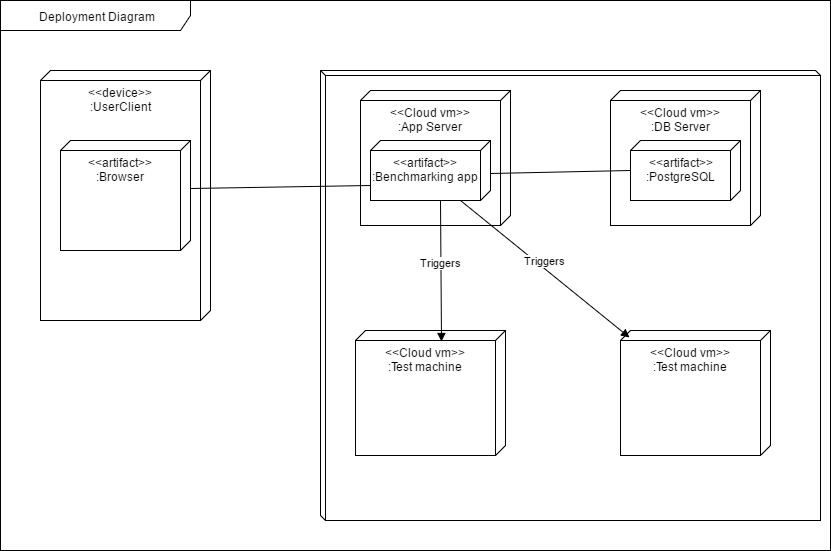
\includegraphics[width=\linewidth]{Deployment Diagram.jpg}
  \caption{Deployment Diagram.}
  \label{fig:Deployment Diagram}
\end{figure}



\end{document}

